\documentclass[tikz]{standalone}

\usepackage{amsmath}
\usepackage{lmodern}
\usepackage{pgfplots}
\usepackage{physics}

\definecolor{exotic orange}{RGB}{255,128,0}
\definecolor{exotic green}{RGB}{0,102,102}
\definecolor{exotic blue}{RGB}{67,132,161}
\definecolor{exotic red}{RGB}{250,86,86}

\pgfplotsset{compat=1.17}
\usepgfplotslibrary{groupplots}
\usetikzlibrary{arrows.meta}

\begin{document}
	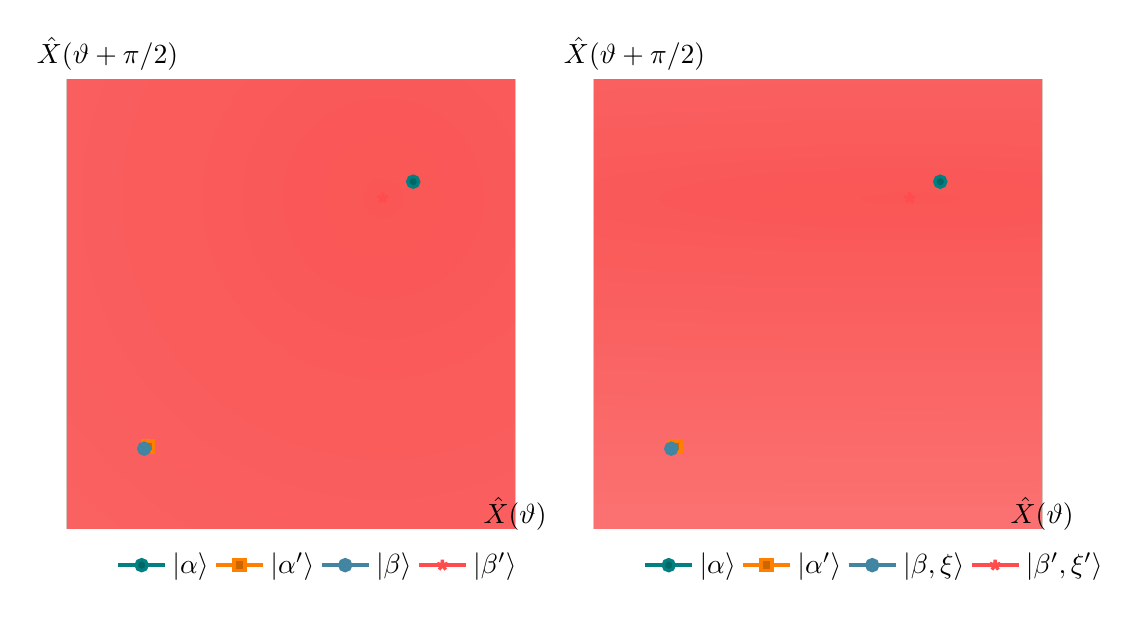
\begin{tikzpicture}
		\begin{groupplot}[
			group style={
				group name=plot,
				group size=2 by 1,
				vertical sep=1ex,
			},
%			width=0.95\linewidth,
			axis lines=center,
			axis equal image,
			xlabel={$\hat{X}(\vartheta)$},
			ylabel={$\hat{X}(\vartheta+\pi/2)$},
			ticks=none,
			xmin=-0.2,
			xmax=+2,
			ymin=-0.2,
			ymax=+2,
			axis line style={thick},
			x label style={
				anchor=north,
			},
			y label style={
				anchor=south,
			},
			cycle list name=exotic,
			legend columns=4,
			legend style={
				at={(axis cs:0,-0.5)},
				anchor=south west,
				draw=none,
			},
		]
			\nextgroupplot
			\draw[thick, -Latex, dotted, gray] (axis cs:1.2,1.2) -- (axis cs:0.35,0.35);
		
			\addplot+[very thick] coordinates {(1.5,1.5)};
			\shadedraw[inner color=exotic green, outer color=exotic green!40, draw=none] (axis cs:1.5,1.5) circle (20);
			
			\addplot+[very thick] coordinates {(0.2,0.2)};
			\shadedraw[inner color=exotic orange, outer color=exotic orange!40, draw=none] (axis cs:0.2,0.2) circle (20);
			
			\addplot+[very thick] coordinates {(0.18,0.19)};
			\shadedraw[inner color=exotic blue, outer color=exotic blue!40, draw=none] (axis cs:0.18,0.19) circle (20);
			
			\addplot+[very thick] coordinates {(1.35,1.42)};
			\shadedraw[inner color=exotic red, outer color=exotic red!40, draw=none] (axis cs:1.35,1.42) circle (20);
			
			\legend{$\ket{\alpha}$,$\ket{\alpha^\prime}$,$\ket{\beta}$,$\ket{\beta^\prime}$};
			
			\nextgroupplot
			\draw[thick, -Latex, dotted, gray] (axis cs:1.2,1.2) -- (axis cs:0.35,0.35);
		
			\addplot+[very thick] coordinates {(1.5,1.5)};
			\shadedraw[inner color=exotic green, outer color=exotic green!40, draw=none] (axis cs:1.5,1.5) circle (20);
			
			\addplot+[very thick] coordinates {(0.2,0.2)};
			\shadedraw[inner color=exotic orange, outer color=exotic orange!40, draw=none] (axis cs:0.2,0.2) circle (20);
			
			\addplot+[very thick] coordinates {(0.18,0.19)};
			\shadedraw[inner color=exotic blue, outer color=exotic blue!40, draw=none] (axis cs:0.18,0.19) ellipse (50 and 6);
			
			\addplot+[very thick] coordinates {(1.35,1.42)};
			\shadedraw[inner color=exotic red, outer color=exotic red!40, draw=none] (axis cs:1.35,1.42) ellipse (50 and 6);
			
			\legend{$\ket{\alpha}$,$\ket{\alpha^\prime}$,$\ket{\beta,\xi}$,$\ket{\beta^\prime,\xi^\prime}$};
		\end{groupplot}
	\end{tikzpicture}
\end{document}